\documentclass[sigconf]{acmart}

\usepackage{graphicx}
\usepackage{hyperref}
\usepackage{todonotes}

\usepackage{endfloat}
\renewcommand{\efloatseparator}{\mbox{}} % no new page between figures

\usepackage{booktabs} % For formal tables

\settopmatter{printacmref=false} % Removes citation information below abstract
\renewcommand\footnotetextcopyrightpermission[1]{} % removes footnote with conference information in first column
\pagestyle{plain} % removes running headers

\newcommand{\TODO}[1]{\todo[inline]{#1}}

\begin{document}
\title{Predicting Profitable Customers in Banking Industry}


\author{Dhanya Mathew}
\orcid{HID328}
\affiliation{%
  \institution{Indiana University}
  \streetaddress{711 N Park Ave}
  \city{Bloomington} 
  \state{Indiana} 
  \postcode{47408}
}
\email{dhmathew@iu.edu}


% The default list of authors is too long for headers}
\renewcommand{\shortauthors}{G. v. Laszewski}


\begin{abstract}
Banks often want to know the profile of their profitable top 1\% or 20\% customers looks like. Conversely, they may also wonder what the general profile is of the customers in the worst 1\% and 20\% of profit. Based on customer's data variables at any given time, a good predictive model can predict which profit group (extremely unprofitable, average, extremely profitable, etc.) customers fall into. This helps financial institutions to better understand what drives the customer profit and accordingly take decisions to sell their products to the right customers. Further down in banking sector, it is a challenge to identify customers who are most likely to repay the loan. Recent big data and machine learning technologies have the potential to predict good customers and open doors for banks to profitable growth. Since the banking sector has evolved over the periods, there are tremendous amount of historical data available to analyze. We show how bank's big data can be analyzed and create a model based on that, to classify customers. In addition to big data technologies, we use machine learning algorithms to build a predictive model to predict creditworthy and uncreditworthy customers from a list of new customers. Random forest classification algorithm is used to achieve this goal.

\end{abstract}

\keywords{i523, HID328, Big Data, Spark, Python, Decision Trees , Random Forest}


\maketitle



\section{Introduction}

Big data as the name implies, refers to large and complex data which continues to grow enormously day by day. Industries like financial firms, in particular, have widely adopted big data analytics to obtain better investment decisions with consistent growth. Recent survey research indicates that 71 percent of firms in the financial services industry at a global level are exploring big data and predictive analytics \cite{accenture-next-generation-financial}. This number continues to grow and sectors like government, business, technology, universities, health-care, finance, manufacturing etc make use of big data to obtain meaningful information using big data technologies \cite{wiki-bigdata}. 

The finance sector contributes to the daily data generation from products and marketing, banking, business, share market etc \cite{how-big-data-has-changed-finance}. Banking is a very sensitive field and any useful insight can make a positive impact on the overall turnover. Historic data analysis and real time data analysis are equally important in banking sector. The era of big data helps financial firms to take quality business decisions related to expanding revenues, managing costs, hiring resources etc, based on effective data analysis which provide access to real-time insights. Data-driven decision making is one of the key advantages of big data technologies.

\subsection{Project Goals}\label{Project goals}

This project aims to help banking sector to identify trustworthy customers. Specifically, help banks to take a decision driven by data, whether to approve or reject a loan application. When a new customer approaches the bank for a loan, banks would be able to identify the customers who are most likely to repay the loan by analyzing the applicant's profile and background information. 

There can be two scenarios of risks associated with the bank's decision. First, if the customer is creditworthy and if the bank rejects the loan, then it is a loss to the bank in terms of interest. Second, if the customer is uncreditworthy and if the bank approves the loan, then it is a loss to the bank in terms of loan amount and interest \cite{psu-site}. Approving loan for an uncreditworthy customer will end up in more financial loss for the bank and accordingly is a greater risk. Hence banks would require a decision rule to follow for whom to approve the loan. With our model, we are trying to mitigate these risks for the banks and contribute to the decision rules. In other words, our model helps to minimize the risks and maximize the profit by understanding the customers.

\subsection{Methods and Technologies Involved}\label{Methods and Technologies Involved}

The goal of most of the big data projects is to analyze the Data and derive knowledge out of it. In other words, data is the input to the model and knowledge is the output. We also follow the same methods and processes for our project. We wrote the project code using Python3. 

\subsubsection{Project Workflow:}

Overall workflow of the project is shown in Figure \ref{fig:Figure1}. 
For this project, we have taken a sample data set of loan applications received by a bank. We explored the data and the requirements of the bank and based on that set the project goals as discussed in the section \ref{Project goals} before starting the project. In the real scenarios, we will not be able to apply analytical methods directly on the raw data as it likely be imperfect and containing irrelevant information. Hence we do data cleaning (data preprocessing) as the first step. We did data cleaning using PySpark. The cleaned data has 1000 customer records with 1 classifier and 20 feature variables.

\begin{figure}[htb]
  \centering
  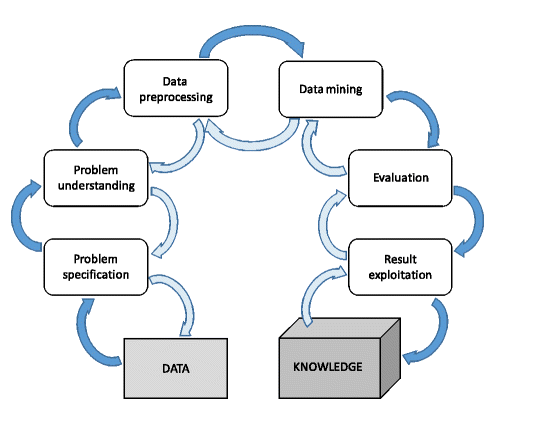
\includegraphics[width=1.0\columnwidth]{project/images/Figure1.png}
  \caption{Project Workflow
  \cite{preprocessing}}
  \label{fig:Figure1} 
\end{figure}

Exploratory analysis like Chi-square test is done to understand the data and feature selection for analysis as part data mining process. We have done graphical representations to show how the actual data is related and what are the direct insights available from the cleaned data set.

Machine learning approaches are used for the data evaluation and to build our predictive model. We develop various models using machine learning algorithms and compare them to identify the best model to choose for our problem solution \cite{sas-machine-learning}. To develop the models we first split the data set into two parts- training data and test data. We defined 2 baseline models, Decision trees and the Random Forest model.  We compare all these models to identify the most effective and least penalty model. We use python as the programming language to build these models and display visualizations for easy comparison and results discussion.

\subsubsection{Python:}

Python version 3 is the programming language used to develop the models and visualizations in this project. Python is a general purpose programming language that is open source, easy to use, faster to write, flexible and powerful. It has a rich set of libraries and utilities for data processing and analytics tasks \cite{python-important-big-data-analytics-applications}. Other important features of Python include the ability to process big data, scalability of applications and easiness to integrate with web applications. 
We use Python libraries like pandas, matplotlib, seaborn and numpy in this project.

\textit{Pandas:} Pandas is one of the most popular libraries in Python. Pandas is used for data manipulation and analysis \cite{pandas}, read data files from different sources, create data frames and some built-in visualizations \cite{dataconomy-python}.

\textit{Matplotlib:} Matplotlib is the library used for plotting arrays and histograms of data in python \cite{Matplotlib}.

\textit{Seaborn:} Seaborn is a Python visualization library used for statistical visualization of data \cite{seaborn}.

\textit{Numpy:} Numpy is Python library which is used to operate mathematical functions on large multi dimensional arrays \cite{numpy}. 

\subsubsection{PySpark:}

Even though Python is powerful to handle complex big data analytic tasks, it alone cannot handle the big data processing. A distributed framework would require to handle a large amount of data. Spark is a distributed computing framework which supports Python \cite{pyspark}.

PySpark is used to carry out the data preprocessing tasks in this project. it is the Python API for Spark.

\subsubsection{Jupyter Notebook:}

Jupyter notebook is an open source web application that allows to edit, run and share Python code and visualizations into a web view. It can be used to modify and re-execute program parts in a flexible way \cite{jupyter}. The files created in Jupyter notebook use extension ''ipynb''. 

\subsubsection{Machine Learning:}

Machine learning enables computers to learn automatically and act accordingly without human assistance or being explicitly programmed. It is an application of Artificial Intelligence. It focuses on computer programs that can access data and learn by itself. Learning process starts by observing the data for patterns and make better decisions in future on the given scenarios \cite{machine-learning}. There are mainly 2 categories of machine learning - Supervised and unsupervised.

\textit{Supervised Machine Learning Algorithms:} Supervised machine learning algorithms enable machines to get trained using a known training data set. Using these labeled examples, supervised learning algorithms can predict future events by applying already learned knowledge. These systems can be used for target definitions for new set of data after required training. Also, it can compare new data input with the intended output and give error indications \cite{machine-learning}. 

\textit{Unsupervised Machine Learning Algorithms:} Unsupervised machine learning algorithms are used when there is not a preferred output and the data is not labeled or classified. It helps to find the hidden patterns in the data. It can describe the hidden structure of the unlabeled data but would not be useful to provide a correct, intended output \cite{machine-learning}. 

There is another categorization of the machine learning algorithms depending on the preferred output. That include \emph{Classification Algorithms} (Used for supervised learning with discrete output), \emph{Regression Algorithms} (Used for supervised learning with continuous output), \emph{Clustering Algorithms} (Unsupervised) etc \cite{wiki-machine-learning}.

We use supervised machine learning approaches in this project. In particular, the classification algorithms - Decision Tree and Random Forest.

\subsubsection{Decision Tree}

Decision Tree is a supervised machine learning algorithm used to solve both classification and regression problems. In decision tree, a trained model with a set of rules will be created based on the training data. The target class or value of a test/new data set will be predicted based on this training rules. Decision Tree algorithm is simple to understand as it uses a tree model representation to solve the problem. It starts from a root node and continues with other decision nodes. Each internal decision nodes corresponds to the feature variables and each leaf nodes corresponds to the class label \cite{decision-tree}. Figure shows the decision tree classifier. 


\begin{figure}[htb]
  \centering
  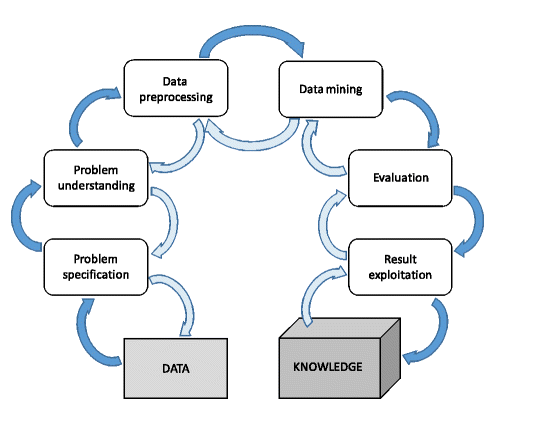
\includegraphics[width=1.0\columnwidth]{project/images/Figure1.png}
  \caption{Project Workflow
  \cite{preprocessing}}
  \label{fig:Figure1} 
\end{figure}

The best attribute will be chosen as the root node. To identify the root node there are 2 methods. They are, \emph{Information Gain} and \emph{Gini Index}. There are statistical approaches to calculate Information gain and Gini index values for each feature variables. Attribute with better value will be considered as the root node and other attributes will be placed in the internal nodes according to the values in recursive order. Step 1 to model the decision tree is placing the root attribute. In step 2, the training data set will be divided into 2 sub data sets in such a way that, both subsets will contain same attribute values for that variable. Step 1 and 2 will be repeated until we reach the leaf nodes with predicted class value \cite{decision-tree}.

\textit{Overfitting:} Overfitting is a practical issue that can happen while building a decision tree. When the algorithm goes deeper and deeper it builds more branches because of the irregularities in data and the prediction accuracy of the model goes down accordingly. There are 2 methods can be used to avoid overfitting issues - \emph{Pre-Pruning} and \emph{Post-Pruning}. In Pre-pruning, we set a threshold value as a goodness measure and if it crosses, further split of the node will be stopped. In Post-Pruning, tree construction continues until all leafs are reached. Pruning will be done if the model shows overfitting issues. Cross-validation data will be used to measure the improvement in this method \cite{decision-tree}.

\subsubsection{Random Forest}

Like Decision Tree, Random Forest algorithm also can be used for classification as well as regression problems. It is a supervised machine learning algorithm. It uses decision tree concept as well but there will be more than one trees in a Random Forest. As the number of trees increases in the Random forest, the accuracy of the prediction also will increase accordingly. Random forest algorithm can handle missing values in the data. Also with more trees in the forest, overfitting issues will not occur in Random Forest algorithm. Figure shows the Random Forest model.

\begin{figure}[htb]
  \centering
  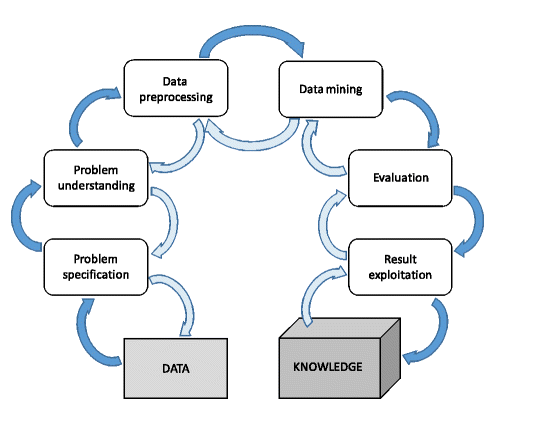
\includegraphics[width=1.0\columnwidth]{project/images/Figure1.png}
  \caption{Project Workflow
  \cite{preprocessing}}
  \label{fig:Figure1} 
\end{figure}

Random Forest algorithm progresses via 2 stages - Random forest creation and Perform prediction. To create the Random Forest, we select a random number of feature variables from the total list of feature variables in the training data and create a Decision Tree out of it. We repeat this process to create desired number of trees. These randomly created trees will form a Random Forest. Figure shows how random forest algorithm works. 

\begin{figure}[htb]
  \centering
  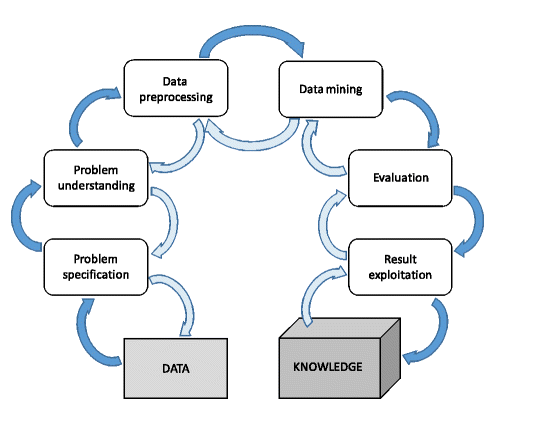
\includegraphics[width=1.0\columnwidth]{project/images/Figure1.png}
  \caption{Project Workflow
  \cite{preprocessing}}
  \label{fig:Figure1} 
\end{figure}

The test data set will be analyzed against the rules developed by each of the trees to predict the output. To predict Random Forest output, the outputs of each of the trees are considered as votes. The top voted output is the final predicted value of the Random Forest.


\subsection{Installations}

Technologies used in this project are discussed in detail in section \ref{Methods and Technologies Involved}. The installation commands on Ubuntu OS for each of these technologies are given in this section. Installations can be done from the Terminal window. 

\begin{enumerate}
  \item Python installation steps for ubuntu OS are available in the askubuntu website \cite{python-installations}.
  \item Install pip to manage the libraries in the Python. Pip is a Python package management software used to install and manage Python libraries. pip can be installed using command ''sudo pip install -U pip'' \cite{pip-package}.   
  \item Install PySpark using command ''sudo pip install pyspark'' \cite{pyspark-installation}.
  \item Install Jupyter notebook using command ''sudo pip install jupyter'' \cite{jupyter-installation}.
   \item Install Pandas using command ''sudo pip install pandas'' \cite{pandas-installation}.
   \item Install matplotlib using command ''sudo pip install matplotlib'' \cite{matplotlib-installation}.
   \item Install seaborn using command ''sudo pip install seaborn'' \cite{seaborn-installation}.
   \item Install numpy using command ''sudo pip install numpy'' \cite{numpy-installation}
\end{enumerate}

All these installation steps are included in a make file referred in appendix \ref{Makefile}.

\section{Data Set}

We used the German Credit data which is publically available in the UCI Machine Learning Repository \cite{uci} and also in the website of PennState Eberly College of Science \cite{psu-site}. Both these sites have the cleaned dataset and not the original one. The dataset that we used in this project (german-credit.csv) is taken from the website of PennState Eberly College of Science \cite{psu-site} and it is uploaded in the Github repository \cite{github}. We recreated the original one from these data sets to understand and try out the data cleaning processes. We start our project with the recreated original data set (credit-data.csv) which is available in the Github repository \cite{github}. 

Dataset includes 1000 customer records with 20 feature variables and a class variable. In the class variable, the actual class of the customer is specified - good or bad. The complete list of data set variables and their description is given in Table \ref{tab:table1}. Figure \ref{fig:Figure2} shows the first 10 rows of the original data set.

\begin{table}
  \caption{Variables and description
  \cite{psu-site}}
  \label{tab:table1}
  \begin{tabular}{cc}
    \toprule
     Variable& Description\\
    \midrule
    Credit& Creditability: Good or Bad\\
    Account Status& Balance of current account\\
    Credit Months& Duration of Credit (month)\\
    Credit History& Payment Status of Previous Credit\\
    Purpose& Purpose of credit\\
    Credit Amount& Amount of credit\\
    Savings& Value Savings or stocks\\
    Employment& Length of current employment\\
    Installment Rate& Installment in \% of current income\\
    Personal Status& Sex and Marital Status\\
    Guarantors& Further debtors\\
    Residence& Duration in Current address\\
    Property& Most valuable available asset\\
    Age& Age in years\\
    Other Installments& Concurrent Credits\\
    Housing& Type of apartment\\
    Credit Cards& No of Credits at this Bank\\
    Occupation& Occupation\\
    Dependents& No of dependents\\
    Telephone& Phone number\\
    Foreign Worker& Foreign worker\\
    \bottomrule
  \end{tabular}
\end{table}


\begin{figure}[htb]
  \centering
  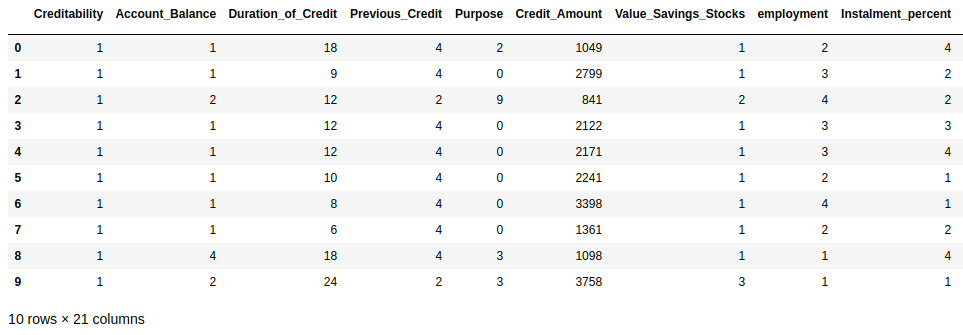
\includegraphics[width=1.0\columnwidth]{project/images/Figure2.png}
  \caption{First 10 rows of original data set
  \cite{github}}
  \label{fig:Figure2} 
\end{figure}



\section{Data Cleansing}

A massive amount of raw data is piling up in the recent years from different sources and it has been continuously getting stored as the storage mechanism is getting cheaper and the storage capacity increases day by day. This raw data cannot be analysed as it is by human or traditional applications, as the processing capacity of traditional tools has been exceeded because of the volume of the data. That is the reason why big data technologies have evolved and they use distributed systems like MapReduce, Spark, Flink etc. Even if we have a big data solution to process the high quantity of raw data, it is not the efficiency and performance of the solution that determines the quality of the knowledge extracted but it depends on the quality of the data as well. The raw data likely to be imperfect and may contain noise, irrelevant information, missing values etc. It is well known that low quality data will lead to low quality knowledge \cite{preprocessing}. Hence data cleaning is the major step to be performed before we continue with data mining algorithms to make sure that we are using a suitable and relevant data set. 

Data cleaning has 2 parts. First part is data preparation and second part is data reduction techniques. 

\subsubsection{Data Preparation}

The data going to the analytics model should be clean and noise free. Hence data preparation part includes tasks like data cleaning, data normalization, data transformation, missing value imputation, data integration and Noise identification. Figure \ref{fig:Figure4} shows the data preparations tasks \cite{preprocessing}.

\begin{figure}[htb]
  \centering
  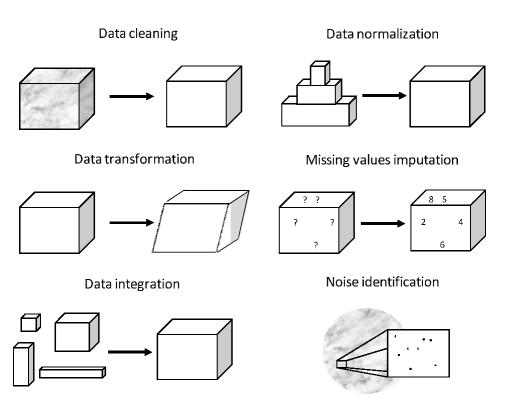
\includegraphics[width=1.0\columnwidth]{project/images/Figure4.png}
  \caption{Data Preprocessing or preparation Tasks
  \cite{preprocessing}}
  \label{fig:Figure4} 
\end{figure}

\subsubsection{Data Reduction Techniques}

To reduce the dimensionality problem and the computational cost, because of a large number of variables and instances in the data set, we try to gather only the required set of quality data. Data reduction techniques include feature selection, instance selection and discretization. Figure \ref{fig:Figure5} shows data reduction techniques \cite{preprocessing}

\begin{figure}[htb]
  \centering
  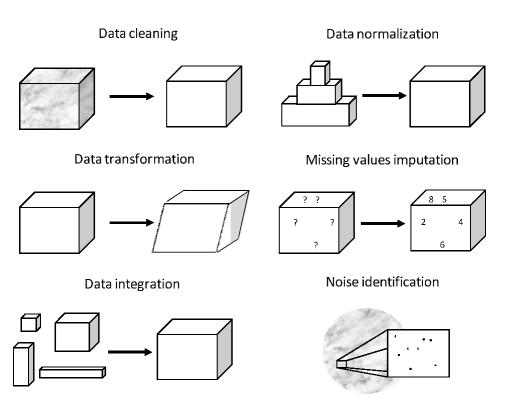
\includegraphics[width=1.0\columnwidth]{project/images/Figure5.png}
  \caption{Data Reduction Approaches
  \cite{preprocessing}}
  \label{fig:Figure5} 
\end{figure}

With respect to our chosen data set, data reduction techniques were already applied to the raw data and 1000 customer records and 21 variables were shortlisted. All these variables are either categorical (like Account-Balance, Previous-credit, purpose etc) or continuous (Duration-of-credit, Installment-percent, dependents). As part of data preparation for our analysis, we transformed the values of categorical variable's from string to scores (numerical values). For example, the variable creditability got 2 values - good and bad. After transformation process, ''good'' got replaced by ''1'' and ''bad'' got replaced by ''0''. Likewise, we gave scores for the values of the variables, Foreign-Worker, Telephone, Previous-Credit, Purpose, Sex-MaritalStatus, Guarantors and Type-apartment. Figure \ref{fig:Figure3} shows first 10 rows from the cleaned data set. 

\begin{figure}[htb]
  \centering
  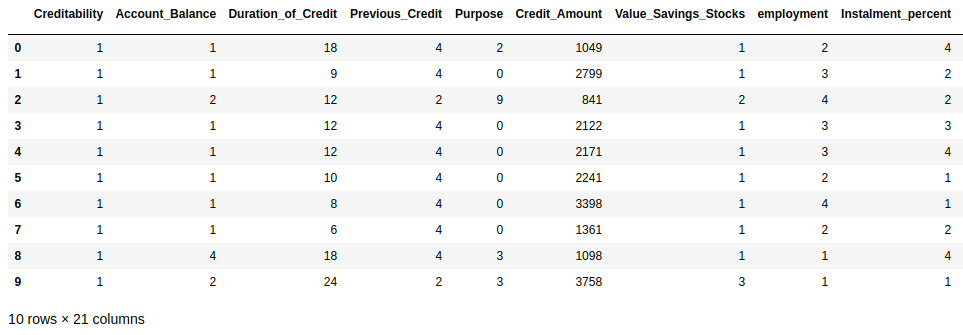
\includegraphics[width=1.0\columnwidth]{project/images/Figure3.png}
  \caption{First 10 rows of cleaned data set
  \cite{psu-site}}
  \label{fig:Figure3} 
\end{figure}


\section{Data Analysis}

Big data analysis is the process of obtaining knowledge by analyzing and understanding hidden patterns, market trends, unknown correlations, customer preferences and other relevant information from large and varied datasets \cite{bigdata-analytics}. Big data analytics methods include exploratory analysis, data mining, predictive analytics, machine learning, deep learning etc. The results of the analysis can be visualized using tools like Tableau, Infogram, Plotly etc or by using python scripts. This project utilizes methods like exploratory analysis, predictive analysis, machine learning algorithms and visualizations of results using python scripts.

\subsection{Exploratory Analysis}

Exploratory analysis is basically to explore the data and understand what it actually contains. It is an approach to summarize the general characteristics of the data set before we attempt to model it. Statistical methods or direct visualizations can help in data exploration \cite{exploratory-analysis}. 

\subsubsection{Direct Visualization}

After data preprocessing, our dataset includes 1000 customer records with 20 feature variable and 1 class variable. Feature variable values can be visualized to understand the characteristics and how they are related to each other - proportionally or inversely. 

Figure shows the histogram of credit amount disbursed with respect to frequency. From this diagram we understand that most of the customers requested for loans for upto 2500 German Marks. The number of customers decreases as the loan amount increases. And very few customers fall under the loan amount category over 10000 German Marks. 

\begin{figure}[htb]
  \centering
  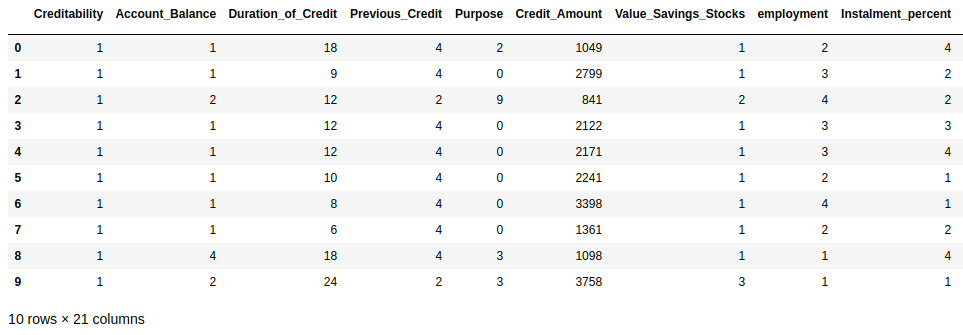
\includegraphics[width=1.0\columnwidth]{project/images/Figure3.png}
  \caption{First 10 rows of cleaned data set
  \cite{psu-site}}
  \label{fig:Figure3} 
\end{figure}

Figure and Figure shows the credit amount availed by bad customers and good customers respectively. The trend is almost same that, maximum customers from both the classes fall under the category of upto 2500 German Marks. But there is a noticeable difference in the number of customers under 12500 range. Bad rated customers are more at this category.

\begin{figure}[htb]
  \centering
  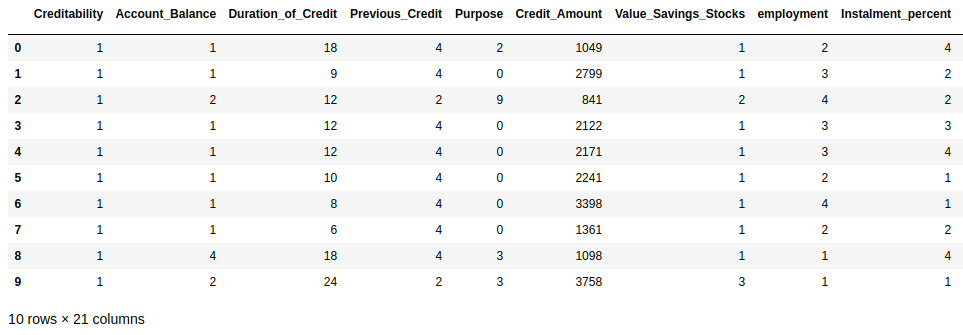
\includegraphics[width=1.0\columnwidth]{project/images/Figure3.png}
  \caption{First 10 rows of cleaned data set
  \cite{psu-site}}
  \label{fig:Figure3} 
\end{figure}

\begin{figure}[htb]
  \centering
  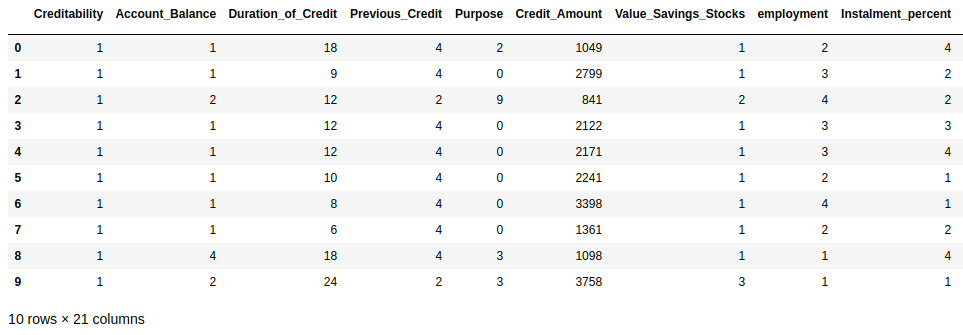
\includegraphics[width=1.0\columnwidth]{project/images/Figure3.png}
  \caption{First 10 rows of cleaned data set
  \cite{psu-site}}
  \label{fig:Figure3} 
\end{figure}

Figure shows the duration of credit in months vs. number of customers. From this graph we can understand that maximum number of customers opted for 10 to 15 months duration.

\begin{figure}[htb]
  \centering
  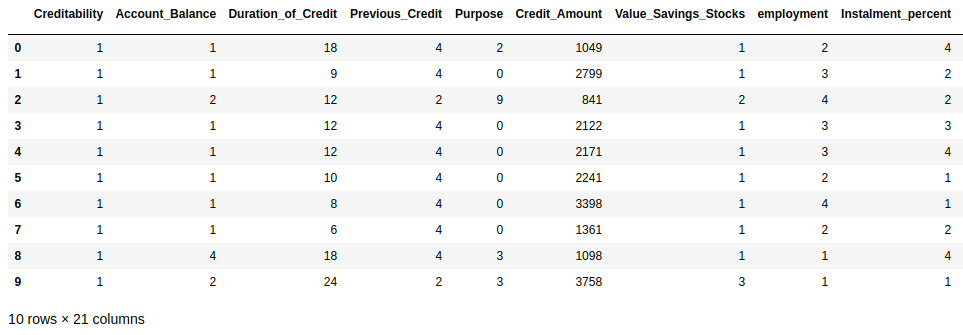
\includegraphics[width=1.0\columnwidth]{project/images/Figure3.png}
  \caption{First 10 rows of cleaned data set
  \cite{psu-site}}
  \label{fig:Figure3} 
\end{figure}

Figure and Figure shows the duration of credit in months vs number of customer bad customers and good customers respectively. It shows that there is not much difference in the trend.

\begin{figure}[htb]
  \centering
  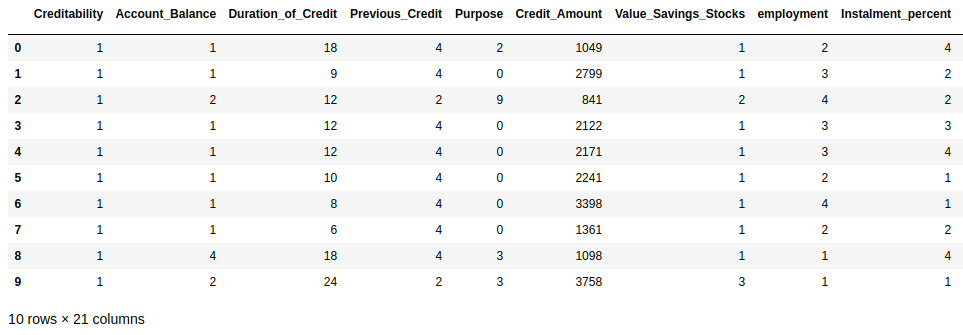
\includegraphics[width=1.0\columnwidth]{project/images/Figure3.png}
  \caption{First 10 rows of cleaned data set
  \cite{psu-site}}
  \label{fig:Figure3} 
\end{figure}

\begin{figure}[htb]
  \centering
  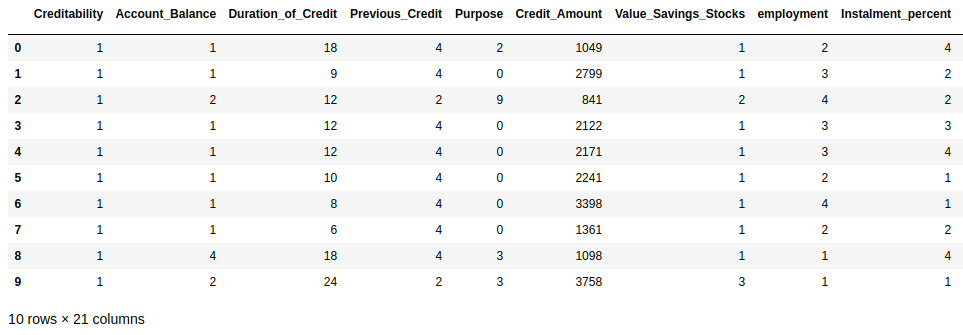
\includegraphics[width=1.0\columnwidth]{project/images/Figure3.png}
  \caption{First 10 rows of cleaned data set
  \cite{psu-site}}
  \label{fig:Figure3} 
\end{figure}

Figure shows how customers are scattered with respect to age. Most of the borrowers fall the age group of 23 to 28.

\begin{figure}[htb]
  \centering
  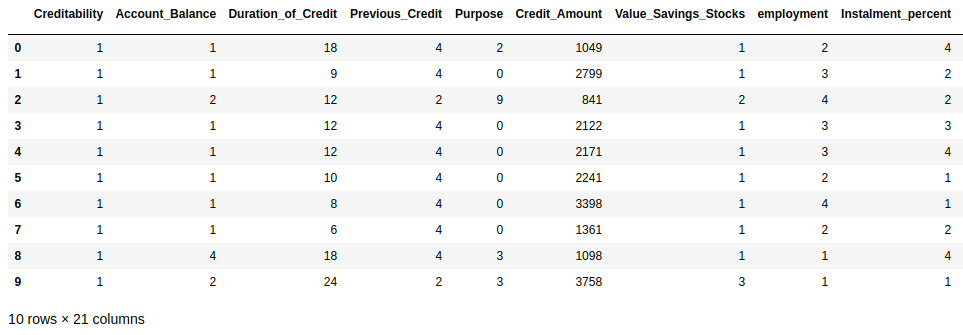
\includegraphics[width=1.0\columnwidth]{project/images/Figure3.png}
  \caption{First 10 rows of cleaned data set
  \cite{psu-site}}
  \label{fig:Figure3} 
\end{figure}

\subsubsection{Data Classification}:

We have one class variable ''Creditability'' to classify the customers. We could extract this class information from dataset using PySpark Python script ''GroupBy''. Figure shows the output of the script.

\begin{figure}[htb]
  \centering
  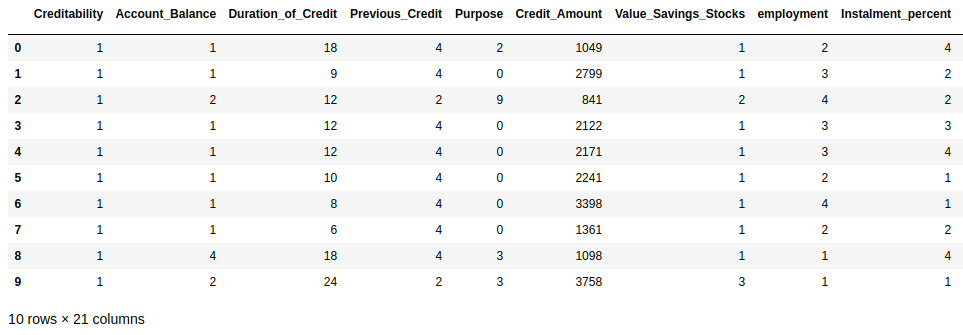
\includegraphics[width=1.0\columnwidth]{project/images/Figure3.png}
  \caption{First 10 rows of cleaned data set
  \cite{psu-site}}
  \label{fig:Figure3} 
\end{figure}

Customers in our dataset are classified into 2 classes - Good (1 = Creditworthy) and Bad (0 = Uncreditworthy). We have 700 customers in the Good class and 300 customers in the Bad class.


\subsubsection{Interquartile Range}:

Interquartile Range is statistical method to measure the variability of the data. This will be applicable only for the continuous variables (Credit-amount, Duration of credit and Age). The rank-ordered data will be divided into 4 equal parts called quartiles. Values are called the First (Q1) Second (Q2) and Third (Q3) quartiles. Q2 is the Median value of the dataset \cite{stat-trek-statistics}.

We used pandas quantile function to extract this information for all the continuous variables.

Figure shows the variability of Credit-Amount.

\begin{figure}[htb]
  \centering
  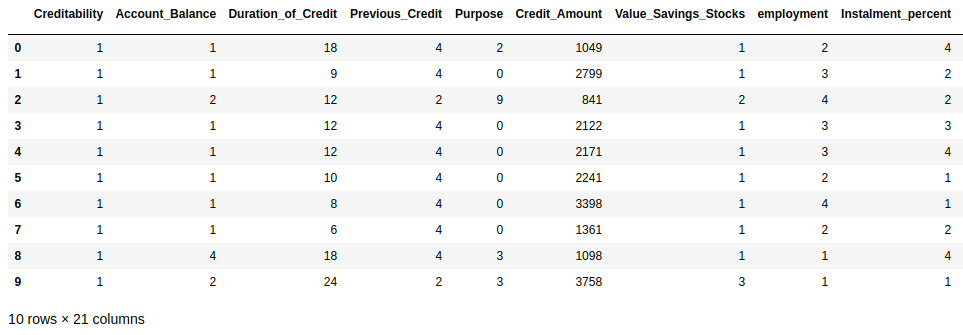
\includegraphics[width=1.0\columnwidth]{project/images/Figure3.png}
  \caption{First 10 rows of cleaned data set
  \cite{psu-site}}
  \label{fig:Figure3} 
\end{figure}

Figure shows the variability of Duration of credit.

\begin{figure}[htb]
  \centering
  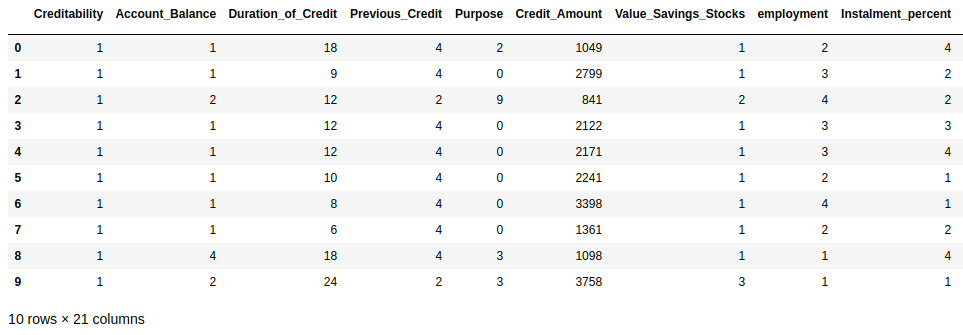
\includegraphics[width=1.0\columnwidth]{project/images/Figure3.png}
  \caption{First 10 rows of cleaned data set
  \cite{psu-site}}
  \label{fig:Figure3} 
\end{figure}

Figure shows the variability of Age.

\begin{figure}[htb]
  \centering
  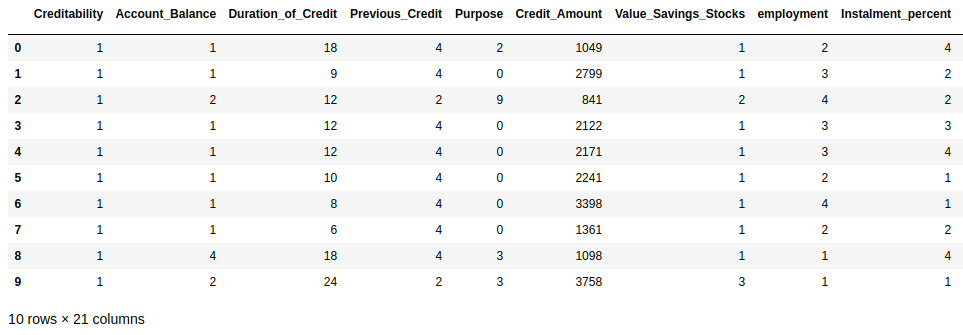
\includegraphics[width=1.0\columnwidth]{project/images/Figure3.png}
  \caption{First 10 rows of cleaned data set
  \cite{psu-site}}
  \label{fig:Figure3} 
\end{figure}

\subsubsection{Cross-Tabulation}

Cross-Tabulation is a statistical method used to compare the relationship between categorical variables. In our scenario we examine the relationship of the categorical variables with the class variable ''creditability''. We create a \emph{contingency table} which displays the frequency of categorical variables with respect to the class \cite{cross-tabulation}. 

\begin{figure}[htb]
  \centering
  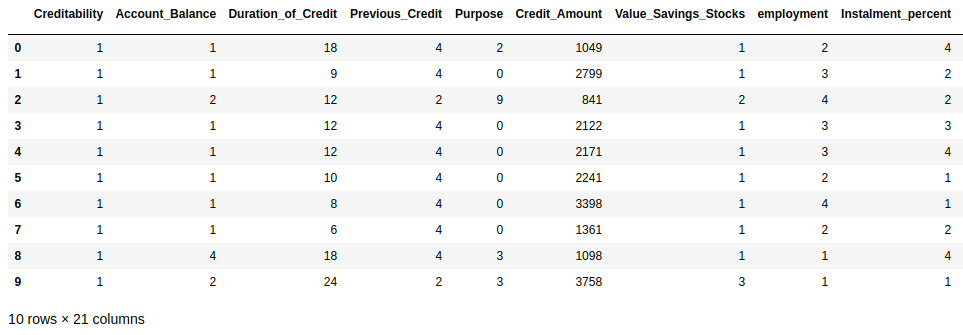
\includegraphics[width=1.0\columnwidth]{project/images/Figure3.png}
  \caption{First 10 rows of cleaned data set
  \cite{psu-site}}
  \label{fig:Figure3} 
\end{figure}

Figure shows the contingency table created for the variable sex-marital status against class. It shows the number of good and bad customers distributed among the 4 categories of the variable sex-marital status. Category ''male: married / widowed'' has the maximum number of Good customers. Contingency tables are used to create the Chi-square values.

\subsubsection{Test of Independence}

We need to identify the features that are closely related to the class/credit rating to build a predictive model. We do a test of independence on all our feature variables to identify the the ones to be selected for data modelling. The method we use to do the test of Independence is the Chi-squared test. The output of the Chi-squared test is the input to the Logistical Regression Algorithm. Variables which are not related to the class variable will be discarded from further analysis of Logical Regression. 

\textit{Pearson's Chi-squared test:}

Chi squared test is used to determine the significant difference between expected values and observed values in one or more categories. There are 2 types of Chi-squared test - Goodness of Fit and Test for Independence. 

We use the second method - \emph{Test of Independence}. It compares 2 variables in a contingency table to check if they are related. In other words, it examines if the distributions of categorical variables are different from one another. 

The formula to see the chi-square value is,

\begin{equation}
X{_c}{^2}=\sum\frac{(O{_}i-E{_}i)^2}{E{_}i}
\end{equation}

Where, ''c'' is the degrees of freedom, ''O'' is the observed value and ''E'' is the expected value.

If the calculated value is small that means, the variables are related. If the value is large that means, the data is not related and not fit for analysis \cite{chi-square}.

\texit{p-value:}p-value is the probability value that, when the null hypothesis is true, the chi-square value will be greater that the empirical value of the data. There is a p-value distribution chart available where it is calculated against he significance value, degrees of freedom and chi-square test value \cite{p-value}.

\textit{Degrees of freedom:} Degrees of freedom is the number of scores that can be varied. It is calculated using the formula,

\begin{equation}
Degrees-of-freedom=(r-1)*(c-1)
\end{equation}

The calculated values are shown in figure

\begin{figure}[htb]
  \centering
  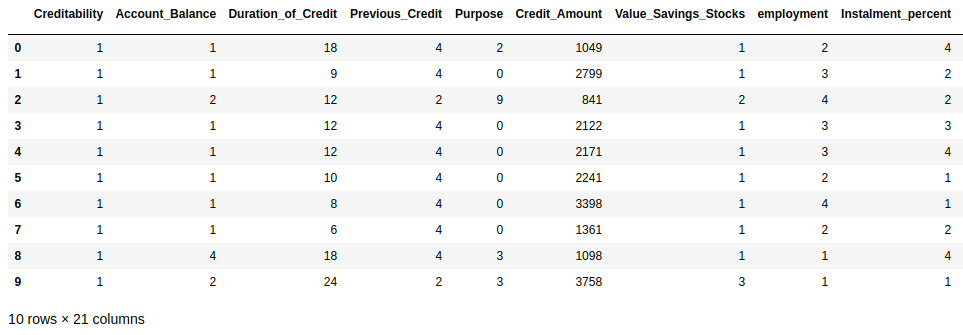
\includegraphics[width=1.0\columnwidth]{project/images/Figure3.png}
  \caption{First 10 rows of cleaned data set
  \cite{psu-site}}
  \label{fig:Figure3} 
\end{figure}


\section{Data Modelling}

\subsection{Penalty Matrix}

\subsection{Baseline Models}

\subsection{Decision Tree Model}

\subsection{Random Forest}

\section{Results}

\subsection{Baseline Model}

\subsection{Decision Tree Model}

\subsection{Random Forest}

\section{Discussion}


\section{Conclusion}

Put here an conclusion. Conlcusions and abstracts must not have any
citations in the section.


\begin{acks}

  The authors would like to thank Dr. Gregor von Laszewski for his
  support and suggestions to write this paper.

\end{acks}

\bibliographystyle{ACM-Reference-Format}
\bibliography{report} 

\appendix

\section{Project References}
\subsection{Makefile}\label{Makefile}

Make file is created assuming that the target system has Python3 installed already.

\subsection{Data Set}
\subsection{Project Code}


\end{document}
